Durant le stage, nous avons commencé par étudier théoriquement le sujet. Comme nous avons étudié l'article de J Ulehla, nous avons commencé par faire une étude bibliographique.

Dans cette partie, nous allons présenter les outils théoriques dans l'ordre d’étude. Ces outils ont été nécessaires pour pouvoir comprendre et mieux implanter le jeu de la forêt.

\subsection{Jeu de Nim}
\label{sub:Jeu de Nim}
  Un jeu de  Nim est un jeu de stratégie pure, c'est-à-dire que ce jeu ne laisse aucune part au hasard et ne permet pas la fin sur une égalité entre les deux joueurs.

  \textit{
    Par exemple, un jeu avec un tas d'allumettes où l'on enlève une ou plusieurs allumettes dans ce tas et où le gagnant est celui qui a retiré la dernière allumette est un jeu de Nim.
  }
  \subsubsection{Jeu de Nim simple}
  \label{subsub: Jeu de Nim simple}
    Un jeu de Nim simple est un jeu de Nim comme défini ci-dessus à ceci près qu'il peut être résolu de façon rapide. Ces jeux ont été résolus par Charles Bouton en 1901\cite{jfji} qui a trouvé un algorithme permettant le gain.

    \textit{
      Le graphe suivant permet de représenter tous les cas possibles pour un jeu de Nim décrit ci-dessus avec un tas à 3 allumettes.
    }
    \begin{figure}[h]
      \centering
        \begin{tikzpicture}[->,>=stealth',shorten >=1pt,auto,node distance=3.5cm, semithick]
          \tikzset{
            state/.style = {shape=rectangle, rounded corners, draw, align=center,
                            top color=white, bottom color=blue!20, text centered}
          }

          \node[initial, state] (3)                    {$3\ allumettes$};
          \node[state]          (f) [below of=3]       {$fin\ du\ jeu$};
          \node[state]          (2) [below right of=f] {$2\ allumettes$};
          \node[state]          (1) [below left of=f]  {$1\ allumette$};

          \path (3) edge (2)
                (3) edge (1)
                (3) edge (f)
                (2) edge (1)
                (2) edge (f)
                (1) edge (f);      
        \end{tikzpicture}
      \caption{Graphe du jeu de Nim simple avec un tas à 3 allumettes}
    \end{figure}

    Le principe de l'algorithme de Bouton est de donner une valeur à chacun des états du graphe représentant le jeu appelé \textit{Nimber}. Dans le cas d'un jeu \`a un tas unique, le \textit{nimber} d'un état est la valeur de l'état elle-même.

    L'attribution de ce \textit{nimber} est récursive, tous les états finaux (un seul état final dans le cas d'un jeu à un tas) ont comme \textit{nimber} 0. Ensuite, pour tout état, le \textit{nimber} est égal au plus petit entier qui n'est pas égal au nimber de chacun de ces fils. Nous pouvons bien facilement voir alors que ce nimber est une interprétation du noyau d'un graphe. En effet, tous les éléments du noyau du graphe d'un jeu seront les éléments ayant un nimber égal a 0.

    \textit {
    Reprenons l'exemple précédent : l’état où le jeu est fini aura comme valeur de nimber 0, ensuite pour l’état avec une allumette, nous aurons comme valeur de nimber 1. Comme nous connaissons le nimber de tous les fils de l’état avec deux allumettes, nous pouvons donner comme valeur de nimber le plus petit entier qui n'est égal à aucune valeur de nimber de ses fils, c'est pourquoi nous lui attribuons la valeur 2. Enfin nous appliquons le même procédé pour l’état avec 3 allumettes et nous lui attribuons la valeur 3.
    }

    Ce \textit{nimber} permet de pouvoir savoir si oui ou non on peut gagner à partir d'une position donnée de jeu.

    Si cette valeur est égale a 0, alors on dit que la position est une \textit{position gagnante}, sinon on dit que cette position est une \textit{position perdante}. Si jamais un joueur commence à partir d'une position perdante, alors il possède une stratégie gagnante, en effet lorsque le joueur est dans une position perdante, alors il y a forcément un état successeur de la position dans laquelle se trouve le joueur qui possède une valeur de nimber valant 0 qui permettra au joueur de gagner.

    Dans le cas contraire, la position dans laquelle se trouve le joueur a un nimber valant 0 alors il n'a pas d’état successeur permettant de gagner. En effet comme la valeur de nimber est le plus petit entier n’étant pas égal aux nimber de ses successeurs, alors il n'y a pas de valeur de nimber de ses successeurs égal a 0. Cela ne permet pas de gagner car jamais le joueur ne pourra atteindre l’état final.

  \subsubsection{Jeu de Nim complexe}
  \label{subsub:Jeu de Nim complexe}

    Un jeu de Nim complexe est un ensemble de jeux de Nim simples. Ils ont été résolus indépendamment par Roland Sprague en 1935 et Patrick Grundy en 1939\cite{tsgE}.

    \textit{
      Par exemple, un jeu de Nim avec plusieurs tas d'allumettes où l'on enlève une ou plusieurs allumettes dans un tas à la fois et où le gagnant est celui qui retire la dernière allumette est un jeu de Nim complexe.
    }

    \textit{
      Le graphe suivant est le graphe d'un jeu avec deux tas de 2 allumettes.
    }

     \begin{figure}[h]
        \centering
        \begin{tikzpicture}[->,>=stealth',shorten >=1pt,auto,node distance=3.5cm, semithick]
          \tikzset{
            state/.style = {shape=rectangle, rounded corners, draw, align=center, top color=white, bottom color=blue!20, text centered}
          }

          \node[initial, state] (22)                     {$2\ allumettes,\ 2\ allumettes$};   
          \node[state]          (21) [below left of=22]  {$2\ allumettes,\ 1\ allumette$};
          \node[state]          (11) [below left of=21]  {$1\ allumette,\ 1\ allumette$};
          \node[state]          (2)  [below right of=22] {$2\ allumettes$};
          \node[state]          (1)  [below of=21]       {$1\ allumette$};
          \node[state]          (f)  [below of=2]        {$final$};
          
          \path (22) edge (21)
                (22) edge (2)
                (21) edge (2)
                (21) edge (1)
                (21) edge (11)
                (11) edge (1)
                (2) edge (1)
                (2) edge (f)
                (1) edge (f); 
      \end{tikzpicture}   
      \caption{Graphe du jeu de Nim complexe avec 2 tas de 2 allumettes}
    \end{figure}

    La résolution de ces jeux est une généralisation de la méthode de résolution des jeux de Nim simples. Le principe est de \textit{diviser pour mieux régner}. En effet, nous divisons le jeu en autant de jeux de Nim simples qu'il y a de tas.

    Comme les jeux de Nim simples, on commence par donner les valeurs de nimber à tous les états du graphe du jeu, puis pour savoir si une position du jeu est gagnante, nous devons faire une opération spéciale appelée \textit{addition de Nim}.

    Cette opération est une addition bit à bit des nimbers en binaire sans retenue. Ceci revient à faire un \textit{ou exclusif} entre les valeurs des nimbers de tous les tas de l’état du jeu.

    Comme le jeu de Nim simple, lorsque le nimber d'une position est égal à 0, on se trouve dans une position gagnante du jeu et dans tous les autres cas, nous nous trouvons dans une position perdante.

    \textit {
      Dans l'exemple d'un jeu avec un tas de 3 allumettes et un tas de 2 allumettes, le joueur qui commencera à jouer à partir de la position (3,2), pourra gagner puisqu'il pourra arriver suite à un mouvement à une position gagnante. Pour savoir quel est ce coup gagnant, il suffit de trouver une valeur pour un des deux tas qui permet d'obtenir un nimber a 0. Ce coup est facile à trouver puisqu'il suffit de retirer une allumette dans le tas avec 3 allumettes (2 ou exclusif 2 est bien égal a 0). Le joueur qui commence a donc bien une stratégie gagnante.
    }

    Cette méthode de résolution est très utilisé puisque nous pouvons trouver une fonction permettant d'attribuer une valeur de nimber en fonction du jeu que nous étudions.

    C'est ce qu'a fait J. Ulehla en 1979 pour trouver une méthode de résolution rapide du jeu de Hackendot de J. Von Neumann.

\subsection{Hackendot}
\label{sub:Hackendot}
  Ce jeu, créé par John Von Neumann et John Horton Conway indépendamment, est un jeu de Nim sur les arbres où l'on retire dans un arbre du jeu le chemin de la racine à un noeud choisi. Le dernier joueur à enlever un nœud du jeu gagne.

  \textit{
    Par exemple, l'ensemble d'arbres suivant est une situation initiale d'un jeu de Hackendot
  }
  \clearpage
  \begin{figure}[h]
        \centering
        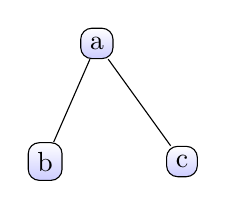
\begin{tikzpicture}[sibling distance=5em, every node/.style = {shape=rectangle, rounded corners, draw, align=center,
                      top color=white, bottom color=blue!20}, right]

          \node {a}
            child{node {b}}
            child{node {c}};
        \end{tikzpicture}
        \hspace{0.2cm}
        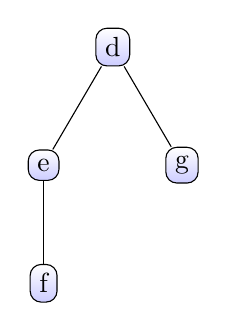
\begin{tikzpicture}[sibling distance=5em, every node/.style = {shape=rectangle, rounded corners, draw, align=center,
                            top color=white, bottom color=blue!20}], left]
            \node{d}
            child{node{e}
              child{node{f}}
            }
            child{node{g}};
        \end{tikzpicture}

  \caption{Forêt d'arbres d'un jeu de hackendot}
  \end{figure}

  La résolution proposée en 1979 par Josef Ulehla est un dérivé de la méthode de résolution des jeux de Nim complexes. En effet, dans son papier \cite{UleHack} Ulehla cherche simplement une fonction qui permettrait de donner une valeur de nimber à une situation de jeu.

  Dans la suite, nous verrons un arbre comme étant un graphe. Le noyau d'un arbre est construit de la même façon que le noyau d'un graphe, tout élément n'ayant pas de fils appartiendra au noyau et tout élément ayant aucun fils n'appartenant pas au noyau appartiendra au noyau.

  Dans son papier, Ulehla défini plusieurs fonctions :
  \begin{enumerate}
    \item \textit{\texttt{l(f)}} qui permet de \textit{dénoyauter}, c'est-à-dire enlever le noyau du graphe du jeu. $l^n(f)$ est la fonction \textit{\texttt{l}} appliquée \textit{n} fois à la forêt \textit{f}.
    \item\textit{\texttt{rip(f)}} (pour Root-ImParity) qui est égal à 0 (resp. 1) si le nombre de racines blanches de \textit{f} est pair (resp. impair).
  \end{enumerate}

  A l'aide de ces deux fonctions, on peut maintenant définir la méthode de résolution du jeu. En effet, pour savoir si on a bien une stratégie gagnante, on commence par \textit{colorer} la foret du jeu. Colorer signifie que tous les nœuds appartenant au noyau sont \textit{blanc} et tous les autres sont \textit{noir}. Ensuite, on \textit{dénoyaute} la forêt, ce qui permet d'obtenir une nouvelle forêt \textit{f'}. Nous répétons ce procédé jusqu’à obtenir une forêt $f^n$ vide. La suite des forêts $f^n$ permet de savoir s'il y a une stratégie gagnante pour la forêt du jeu. En effet, lorsqu'il y a au moins un $rip(f^i)$ avec \textit{i} compris entre \textit{1} et \textit{n} vaut 1, alors il y a une stratégie gagnante.

  Dans cette méthode, la fonction pour donner une valeur de nimber a une position de jeu est la fonction \textit{rip} et l'addition de Nim est la suite des valeurs de \textit{rip} de toutes les forêts $f^n$.

  Enfin, dans sa méthode, Ulehla permet de savoir quel est le coup gagnant. Comme dans la résolution des jeux de Nim complexes, pour trouver quel est le coup gagnant, il suffit de trouver le coup permettant d'avoir une forêt \textit{f''} qui, lorsqu'on applique le procédé décrit précédemment, a un nimber égal à 0 (c'est-à-dire une suite de \textit{rip} égaux à 0).

  Pour trouver ce coup gagnant lorsqu'il existe, il faut prendre la dernière forêt de la suite notée $f^k$ tel \textit{rip($f^k$) = 1}. A partir de cette forêt, on prend l'ensemble des racines blanches et leurs successeurs blancs directs et on regarde quel suppression permet d'obtenir \textit{rip($f^k$) = 0}. On remonte la suite des forêts en prenant à chaque fois l'ensemble constitué du coup gagnant de la forêt précédente et ses successeurs.
  \clearpage
  \textit{
    Reprenons l'exemple du début, la première question que nous nous posons est : est-ce qu'on a une stratégie gagnante en jouant ?
  }

  \begin{figure}[h]
  \centering
    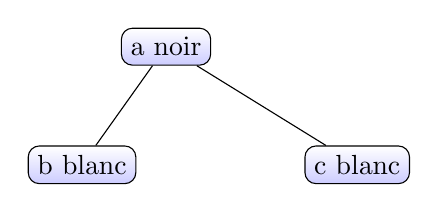
\begin{tikzpicture}[sibling distance=10em, every node/.style = {shape=rectangle, rounded corners, draw, align=center,
                        top color=white, bottom color=blue!20}, right]

      \node {a noir}
        child{node {b blanc}}
        child{node {c blanc}};
    \end{tikzpicture}
    \hspace{0.2cm}
    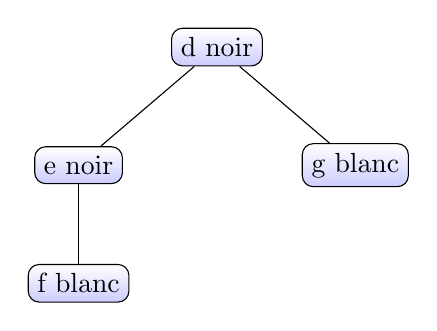
\begin{tikzpicture}[sibling distance=10em, every node/.style = {shape=rectangle, rounded corners, draw, align=center,
                        top color=white, bottom color=blue!20}], left]
        \node{d noir}
        child{node{e noir}
          child{node{f blanc}}
        }
        child{node{g blanc}};
    \end{tikzpicture}

    F rip(F) = 0

    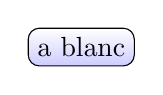
\begin{tikzpicture}[sibling distance=10em, every node/.style = {shape=rectangle, rounded corners, draw, align=center,
                        top color=white, bottom color=blue!20}, right]

      \node {a blanc};
    \end{tikzpicture}
    \hspace{0.2cm}
    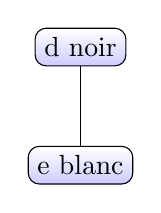
\begin{tikzpicture}[sibling distance=10em, every node/.style = {shape=rectangle, rounded corners, draw, align=center,
                        top color=white, bottom color=blue!20}], left]
        \node{d noir}
        child{node{e blanc}};
    \end{tikzpicture}
    
    l(F) rip(l(F)) = 1
    
    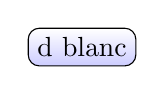
\begin{tikzpicture}[sibling distance=10em, every node/.style = {shape=rectangle, rounded corners, draw, align=center,
                        top color=white, bottom color=blue!20}, right]

      \node {d blanc};
    \end{tikzpicture}
    
    $l^2(F) rip(l^2(F)) = 1$
    
    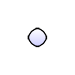
\begin{tikzpicture}[sibling distance=10em, every node/.style = {shape=rectangle, rounded corners, draw, align=center,
                        top color=white, bottom color=blue!20}, right]
      \node {};
    \end{tikzpicture}
    
    $l^3(F) rip(l^3(F)) = 0$
  \caption{Suite des forêts dénoyautées}
  \end{figure}

  \textit{
    Nous savons qu'il existe un coup gagnant en faisant la suite des forêts dénoyautées et que nous devons chercher dans $l^2(F)$. Nous savons que dans cette forêt, il suffit de retirer le nœud \texttt{d} qui permet d'obtenir rip égal à 0.
  }

  \textit{
    Nous cherchons maintenant dans la forêt l(F) quel est le coup permettant d'obtenir un rip égal à 0. Nous savons que dans la forêt précédente, le coup gagnant était \texttt{d} donc ici, nous regardons l'ensemble constitué de \texttt{d, e}.
    Nous voyons que c'est le nœud \texttt{d} qu'il faut supprimer pour avoir un rip égal à 0.
  }

  \textit{
    Enfin, nous appliquons le même procédé à la forêt F et nous trouvons que le coup gagnant est \texttt{g}.
  }
\subsection{Parcours sur les arbres}
\label{sub:Parcours sur les arbres}
\hypertarget{GenArbres}
  Durant l'implantation du jeu de Hackendot, nous nous sommes retrouvé face à une difficulté : comment implanter des arbres quelconques en python ?

  Pour répondre à ce problème, Madame Selmi m'a fourni le travail d'un ancien étudiant\cite{SamWor} qui a utilisé uniquement le parcours préfixe et suffixe sur les arbres et a permis de gérer l’intégralité de ce problème.

  Quelque soit le parcours utilisé, nous regardons de gauche à droite les nœuds dans l'arbre, c'est-à-dire que lorsque nous sommes sur un nœud donné, nous cherchons d'abord à découvrir récursivement tout son fils gauche puis nous allons découvrir son fils droit.

  Tout d'abord, nous avons utilisé le parcours préfixe sur une forêt. Ce parcours est effectué dans l'ordre de \textit{découverte} des nœuds dans la forêt. Nous pouvons obtenir la liste préfixe, notée P, d'un arbre en mettant les nœuds dans l'ordre de découverte d’après le parcours préfixe.

  \textit{ 
    Par exemple, dans l'arborescence suivante, la liste préfixe est (1, 2, 3, 4)
  }
  \clearpage
  \begin{figure}[h]
    \centering
    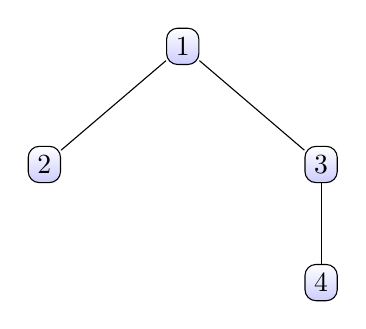
\begin{tikzpicture}[sibling distance=10em, every node/.style = {shape=rectangle, rounded corners, draw, align=center,
                        top color=white, bottom color=blue!20}], left]
        \node{1}
        child{node{2}}
        child{node{3}
          child{node{4}}
        };
    \end{tikzpicture}
    \caption{Arborescence de liste préfixe (1, 2, 3, 4)}
  \end{figure}

  Ensuite, nous avons utilisé le parcours suffixe sur une forêt. Ce parcours est effectué dans l'ordre de fin de découverte des nœuds dans la forêt. Un nœud est entièrement découvert lorsque nous avons entièrement exploré tous ses successeurs. Grâce à ce parcours, nous pouvons créer la liste suffixe, notée S, en mettant dans l'ordre de découverte par rapport à ce parcours les nœuds de la forêt.

  \textit{
    Dans l'exemple précédent, la liste suffixe de l'arborescence est (2, 4, 3, 1)
  }

  Nous avons aussi défini les listes \textit{S(n)} et $P^{-1}(n)$ comme étant respectivement la liste suffixe à partir d'un nœud n et la liste des nœuds du début de la liste préfixe jusqu'au nœud n.

  \textit{
    Dans l'exemple précédent, prenons le nœud 2, alors la liste S(2) est la liste (4, 3, 1) et la liste $P^{-1}(2)$ est la liste (1).
  }

  Grâce à ces différentes listes, nous avons pu connaitre le père direct d'un nœud \textit{n} de la forêt. En effet, nous remarquons que le père direct du nœud est le premier élément de \textit{S(n)} commun à la liste $P^{-1}(n)$ .

  Nous avons aussi remarqué que tous les nœuds du chemin de la racine à un nœud \textit{n} étaient tous les nœuds commun à la liste S(n).

  Durant ce stage, la preuve de ces deux éléments a été fournie.

  Ces listes préfixes et suffixes ont été utilisées sur des mots de Dyck générés de façon aléatoire avec une grammaire dont les règles sont :

  \begin{itemize}
    \item S -> () qui permet de créer une racine sans fils
    \item S -> ()S qui permet de créer une racine avec une seconde arborescence
    \item S -> (S) qui permet de créer une racine avec un sous arbre
    \item S -> (S)S qui permet de créer une racine avec un sous arbre et une seconde arborescence
  \end{itemize}

  \textit{Par exemple, dans l'arborescence précédente, le mot de Dyck est généré est : \texttt{(()(()))}}

\subsection{Jeu de Chomp}
\label{sub:Jeu de Chomp}

Le dernier jeu que nous avons étudié est le jeu de Chomp revisité. Comme le Chomp, nous jouons sur une tablette carrée ou rectangle, mais nous avons cependant modifié les règles pour faciliter le jeu. Nous devons choisir une case et supprimer soit la ligne, soit la colonne de la case choisie. Le dernier joueur à enlever une case est le vainqueur.

\textit{
  Voici une situation de jeu avec une tablette rectangle 3x4
}

\begin{figure}[h]
  \centering
  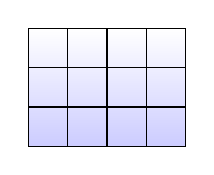
\begin{tikzpicture}
    %carre principal
    \fill[ top color=white, bottom color=blue!20] (0,0) -- (0, 1.5) -- (2,1.5) -- (2,0) --(0,0);
    \draw (0,0) -- (0, 1.5) -- (2,1.5) -- (2,0) --(0,0);
    %lignes
    \draw (0,0.5) -- (2,0.5);
    \draw (0,1) -- (2,1);
    %colonnes
    \draw (0.5, 0) -- (0.5, 1.5);
    \draw (1, 0) -- (1, 1.5);
    \draw (1.5, 0) -- (1.5, 1.5);
  \end{tikzpicture}
  \caption{Situation de jeu du Chomp}
 
\end{figure}
Au démarrage, ce jeu devait être sur les polyominos convexe (sans trou) cependant, nous nous sommes rendus compte que travailler sur une tablette ou sur un polyomino revenait au même. En effet, nous pouvons voir facilement qu'un polyomino convexe est compris dans une tablette, c'est pourquoi nous avons généralisé directement sur une tablette.

Ensuite, nous avons cherché à diviser ce jeu de façon à pouvoir utiliser le théorème de Sprague-Grundy, nous avons donc pensé que le but était de calculer le nombre de lignes et de colonnes. Nous avons pensé que si le nombre de lignes ou le nombre de colonnes était impair, le coup était gagnant.

Puis nous avons implanté le jeu avec cette idée, cependant nous sommes tombé face à un contre exemple. C'est pourquoi nous avons essayé de faire en sorte de revoir la façon de calculer si le coup est gagnant. Nous avons donc pensé que lorsque nous avons plusieurs composantes connexes, nous pouvons les mettre sous la forme d'une tablette avec comme nombre de ligne la somme du nombre de ligne de toutes les composantes connexes, et de la même façon le nombre de colonnes la somme des colonnes de toutes les composantes connexes.

A la fin de ce stage, nous n'avons pas réussi à savoir comment faire pour savoir s'il existe une stratégie gagnante à partir d'une position de jeu donnée, et si oui, comment calculer le coup gagnant.

Cependant, nous avons conjecturé que, pour une position donnée, le nimber valait :
\begin{itemize}
  \item \texttt{m} dans le cas d'une tablette 1xm ou mx1 (prouvé)
  \item \texttt{0} si la tablette est de la forme 2nx2m (prouvé)
  \item \texttt{1} si dans une tablette nxm avec m ou n impair m + n est impair
  \item \texttt{2} sinon
\end{itemize}
  Nous avons mis au point un petit programme permettant la vérification de cette conjecture et à ce jour, nous n'avons pas trouvé de contre exemple.
